\documentclass[11pt,a4paper]{article}
\usepackage[T1]{fontenc}
\usepackage[margin=2.3cm]{geometry}
\usepackage{amsmath,amssymb}
\usepackage{graphicx}
\usepackage[dvipsnames]{xcolor}
\usepackage{enumitem}
\usepackage[colorlinks=true,linkcolor=blue,urlcolor=blue]{hyperref}
\setlength{\parskip}{0.6em}
\setlength{\parindent}{0pt}
\begin{document}

\begin{center}{\LARGE\bfseries opencalculus}\\[0.4em]{\large See derivatives and integrals as slopes and areas on a moving car's graph.}\\[0.2em]\small PAN IIT OSS explainer \textbullet{} secondary school to diploma / undergraduate (levels 3-5)\end{center}

\section*{Why this exists}
Calculus is the mathematics of change and accumulation. This explainer follows a moving car: the slope of its distance graph is its speed and the area under its speed graph is the distance it covers, then shows how computers estimate both and how large their errors are.

\section*{The end goal}
See derivatives and integrals as slopes and areas on a moving car's graph. The end goal is to see derivatives and integrals as slopes and areas on a moving car's graph. The same ideas drive physics (velocity, work, charge), engineering (signals, control) and data science (rates and totals from measurements).

\section*{How the five sessions build up}
\begin{enumerate}[nosep]
\item \textbf{Session 1: Slope is speed, area is distance} (Level 1, conceptual interactive model, 60 min).
\item \textbf{Session 2: Derivative and integral as limits} (Level 2, mathematical engineering model, 75 min).
\item \textbf{Session 3: Numerical slopes and areas, and their errors} (Level 3, simulation and validation, 90 min).
\item \textbf{Session 4: Romberg integration: far more accuracy from the same function values} (Level 3, simulation and validation, 90 min).
\item \textbf{Session 5: Gaussian quadrature: choosing where to sample} (Level 3, simulation and validation, 90 min).
\end{enumerate}

\section{Session 1: Slope is speed, area is distance}

\subsection*{A. Real-world problem}
A car's speedometer tells you how fast you go but not how far you have come; its odometer tells you how far but not how fast. If you only had a record of one of them, could you rebuild the other? That question is the whole of calculus in disguise: going from distance to speed is differentiation, going from speed to distance is integration. In this session you do both with nothing but slopes and areas.

\subsection*{B. Concept and theory}
Speed is distance divided by time. On a distance-time graph, 'distance divided by time' is rise over run, the slope. When the speed changes, the slope changes from moment to moment: the speed at a moment is the slope of the tangent line touching the curve there. Going the other way, distance equals speed times time. On a speed-time graph that is width times height, the area of a rectangle; if the speed changes we cut the time into slices and add up the areas (a trapezoid for a straight-line change). The unit of the area is s * m/s = m. Our car starts at rest and its speed is known at 0, 2, 4 and 6 s, with straight lines in between.

\begin{itemize}[nosep]
\item t: time since the start (s)
\item v(t): speed of the car at time t (m/s)
\item x(t): distance travelled since the start, up to time t (m)
\item slope: rise over run of the distance graph (m/s)
\item area: area under the speed graph (m)
\end{itemize}

\begin{equation*}
v=\frac{\Delta x}{\Delta t}\quad\text{(slope of the distance graph)}
\end{equation*}

\begin{equation*}
\Delta x=\frac{v_1+v_2}{2}\,\Delta t\quad\text{(area of one trapezoid under the speed graph)}
\end{equation*}

\begin{equation*}
x(t)=\text{area under }v\text{ from }0\text{ to }t,\qquad v(t)=\text{slope of }x\text{ at }t
\end{equation*}

\begin{center}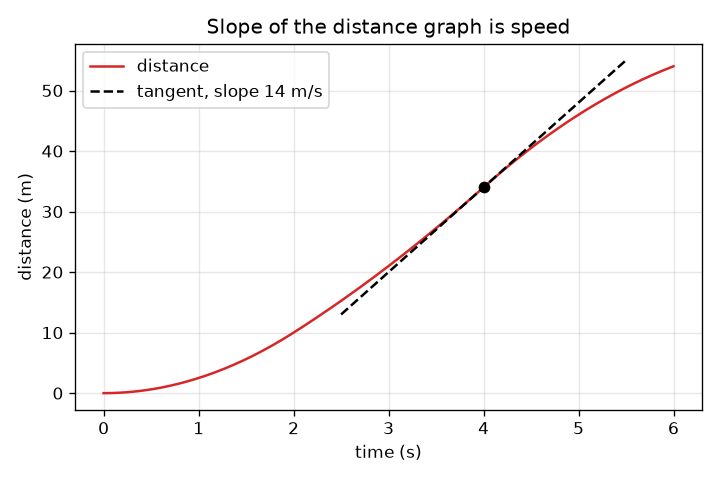
\includegraphics[width=0.85\linewidth]{figures/s01_distance_slope.png}\\\small Distance against time: the tangent at 4 s has slope 14 m/s, the speed.\end{center}

\subsection*{E. Worked example}
A car starts at rest and has speeds 10, 14 and 6 m/s at t = 2, 4 and 6 s, with straight lines between. Find the distance at each of those times, then the speed at t = 3 s and the slope of the distance graph there.
\begin{enumerate}[nosep]
\item Slice 1 (0 to 2 s): trapezoid with sides 0 and 10 m/s and width 2 s: (0 + 10)/2 * 2 = 10 m.
\item Slice 2 (2 to 4 s): (10 + 14)/2 * 2 = 24 m, so the distance at 4 s is 10 + 24 = 34 m.
\item Slice 3 (4 to 6 s): (14 + 6)/2 * 2 = 20 m, so the distance at 6 s is 54 m.
\item Speed at t = 3 s: half way between 10 and 14 m/s is 12 m/s.
\item Slope of the distance graph at 3 s: the distance changes by about 12 m for each second there, so the slope is 12 m/s, the same number. Unit check: m / s = m/s.
\end{enumerate}
\textbf{Answer.} Distances 10 m, 34 m and 54 m at 2, 4 and 6 s; speed 12 m/s at 3 s, equal to the slope of the distance graph there.

\subsection*{F. Questions}
\begin{enumerate}[nosep]
\item \textbf{Conceptual.} A friend says 'the speed graph is flat, so the car is not moving'. Is that right? What does a flat distance graph mean?
\item \textbf{Numerical.} A car has speeds 0, 12, 12 and 6 m/s at t = 0, 2, 4 and 6 s, with straight lines between. Find the total distance in 6 s and the average speed. Check the units.
\item \textbf{Graph and simulation interpretation.} In the distance graph of the car from the worked example (speeds 10, 14, 6 m/s), where is the curve steepest and what is its slope there? What is the slope at the end, t = 6 s?
\item \textbf{Design and optimisation challenge.} Design: choose the speeds at 2, 4 and 6 s (each at most 20 m/s, the limit of this exercise) so that the car covers at least 90 m in 6 s. Find a choice that works and one that fails, and say what you would trade off.
\end{enumerate}

\section{Session 2: Derivative and integral as limits}

\subsection*{A. Real-world problem}
A car's position is x(t) = 3 t\textasciicircum{}2 + 2 t metres, with t in seconds. What are its velocity and acceleration at 2 s, and are the units of every term sensible? Then a harder question: when a driver brakes, how far does the car go before it stops, and how fast can it be going if it must stop within 40 m?

\subsection*{B. Concept and theory}
The slope between two moments t and t + h is the secant slope (x(t + h) - x(t)) / h. As h gets smaller the secant slope settles on one number: the derivative x'(t), the slope of the tangent line. This 'settling' is called a limit. For x = 3 t\textasciicircum{}2 + 2 t at t = 2 the secant slope is 14 + 3 h, which tends to 14 m/s as h tends to 0. Rules: the derivative of c t\textasciicircum{}n is c n t\textasciicircum{}(n-1); of sin t is cos t; of e\textasciicircum{}t is e\textasciicircum{}t. Velocity is the derivative of position and acceleration is the derivative of velocity. For the integral, cut [a, b] into n slices of width dt = (b - a)/n and add up (height) * dt for each slice; as n grows the sum settles on the integral. The fundamental theorem says the integral of v from a to b equals x(b) - x(a) when v = x', so differentiating and integrating undo each other. Units: each term of x = 3 t\textasciicircum{}2 + 2 t must be in metres, so the 3 is in m/s\textasciicircum{}2 and the 2 in m/s. Braking: a steady slowdown a means the speed falls linearly from v0 to 0 in T = v0 / a, and the distance is the area of the triangle v0 T / 2 = v0\textasciicircum{}2 / (2 a). This is a simplified model: real braking depends on tyres, road and load and is not personal driving advice.

\begin{itemize}[nosep]
\item x(t): position of the car (m)
\item v(t) = x'(t): velocity (m/s)
\item a = v'(t): acceleration (m/s\textasciicircum{}2)
\item h: gap between the two moments of a secant (s)
\item n, dt: number and width of rectangles (no unit, s)
\item v0: speed when braking starts (m/s)
\item t\_r: driver reaction time before braking starts (s)
\end{itemize}

\begin{equation*}
x'(t)=\lim_{h\to 0}\frac{x(t+h)-x(t)}{h}
\end{equation*}

\begin{equation*}
\frac{d}{dt}\left(c\,t^n\right)=c\,n\,t^{n-1},\qquad \frac{d}{dt}\sin t=\cos t,\qquad \frac{d}{dt}e^t=e^t
\end{equation*}

\begin{equation*}
\int_a^b v(t)\,dt\approx\sum_{k=0}^{n-1}v(t_k)\,\Delta t,\qquad \Delta t=\frac{b-a}{n}
\end{equation*}

\begin{equation*}
\int_a^b x'(t)\,dt=x(b)-x(a)
\end{equation*}

\begin{equation*}
d_{\mathrm{stop}}=v_0\,t_r+\frac{v_0^2}{2a}
\end{equation*}

\begin{center}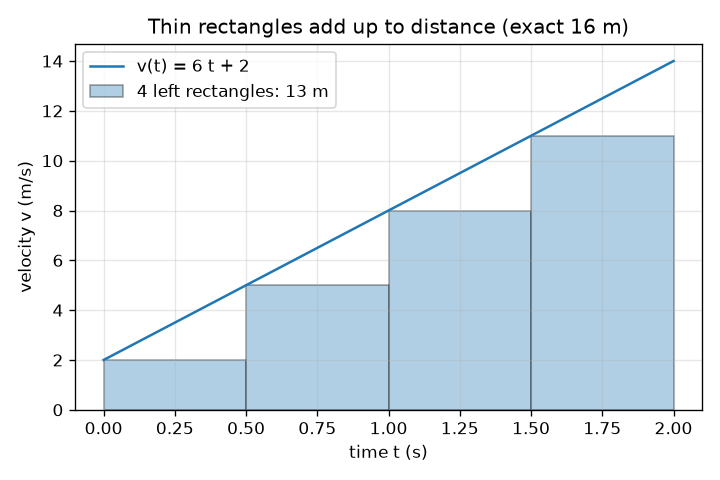
\includegraphics[width=0.85\linewidth]{figures/s02_riemann_rectangles.png}\\\small Four left rectangles under v = 6 t + 2: 13 m against the exact 16 m.\end{center}

\subsection*{E. Worked example}
For x(t) = 3 t\textasciicircum{}2 + 2 t (metres), find the velocity and acceleration at t = 2 s with units, check the derivative with secant slopes, and check the fundamental theorem on [0, 2] with rectangles.
\begin{enumerate}[nosep]
\item Position: x(2) = 3 * 4 + 2 * 2 = 12 + 4 = 16 m.
\item Velocity by the rule: v(t) = 6 t + 2, so v(2) = 14 m/s. Units: 6 is m/s\textasciicircum{}2 and times t (s) gives m/s; 2 is m/s.
\item Acceleration: a = v' = 6 m/s\textasciicircum{}2, constant.
\item Secant check at t = 2: slope = (x(2 + h) - x(2)) / h = 14 + 3 h, so h = 1 gives 17, h = 0.1 gives 14.3, h = 0.001 gives 14.003: tending to 14 m/s.
\item Fundamental theorem: the integral of v from 0 to 2 equals x(2) - x(0) = 16 m. Four left rectangles of width 0.5 s: heights v(0), v(0.5), v(1), v(1.5) = 2, 5, 8, 11 m/s, sum 26 * 0.5 = 13 m (below 16, as the curve rises); four midpoint rectangles give 16 m exactly because v is a straight line.
\end{enumerate}
\textbf{Answer.} x(2) = 16 m, v(2) = 14 m/s, a = 6 m/s\textasciicircum{}2; the secant slopes tend to 14 m/s and the rectangle sums tend to 16 m.

\subsection*{F. Questions}
\begin{enumerate}[nosep]
\item \textbf{Conceptual.} Why does the secant slope never equal the tangent slope exactly for h \textgreater{} 0, and why is it still useful to compute it?
\item \textbf{Numerical.} For x(t) = 5 t\textasciicircum{}2 + 4 t (metres), find x, the velocity and the acceleration at t = 3 s, with units, and check that the units of the two coefficients make sense.
\item \textbf{Graph and simulation interpretation.} In the position view with A = 3, B = 2, t = 2, the secant slope with gap h = 2 s is shown. What value do you read, and what happens when you reduce h to 0.1?
\item \textbf{Design and optimisation challenge.} Design: a driver has a reaction time of 0.75 s and the car brakes at a steady 6 m/s\textasciicircum{}2. What is the stopping distance from 25 m/s (90 km/h)? What is the largest speed that stops within 40 m? State two things this simple model leaves out.
\end{enumerate}

\section{Session 3: Numerical slopes and areas, and their errors}

\subsection*{A. Real-world problem}
A data logger gives numbers, not formulas. To get the acceleration or the distance from a speed record you must differentiate and integrate numerically, and every method makes an error. If you halve the step, how much better do you get? Can the step be too small? And when does a method fail entirely? We answer by testing four methods on functions whose exact answers we know.

\subsection*{B. Concept and theory}
Forward difference (f(x + h) - f(x)) / h has error roughly proportional to h (order 1). Central difference (f(x + h) - f(x - h)) / (2 h) has error roughly proportional to h\textasciicircum{}2 (order 2). Trapezoid rule joins neighbouring sample points by straight lines: error proportional to h\textasciicircum{}2 (order 2). Simpson's rule joins triples of points by parabolas: error proportional to h\textasciicircum{}4 (order 4), with an even number of slices. If error = C h\textasciicircum{}p then log(error) = log C + p log h, so on a log-log plot the points fall on a straight line of slope p: that is how we measure the order. For derivatives there is a second error: the computer stores numbers with about 16 digits, so f(x + h) - f(x) loses digits when h is tiny and the round-off error grows like 1e-16 / h. The total error falls and then rises; the best step sits at the bottom of the V. Methods assume the function is smooth; a corner or a narrow spike breaks the assumptions. Everything here is a simplified model with known exact answers, not a validated library.

\begin{itemize}[nosep]
\item h: step size (same unit as x)
\item n: number of slices, h = (b - a) / n (no unit)
\item p: order of a method: error \textasciitilde{} h\textasciicircum{}p (no unit)
\item tol: tolerance asked of the adaptive rule (same unit as the integral)
\item f(x): function being differentiated or integrated (any)
\end{itemize}

\begin{equation*}
f'(x)\approx\frac{f(x+h)-f(x)}{h}\ \ (\text{error}\sim h),\qquad f'(x)\approx\frac{f(x+h)-f(x-h)}{2h}\ \ (\text{error}\sim h^2)
\end{equation*}

\begin{equation*}
\int_a^b f\,dx\approx h\left[\tfrac12 f_0+f_1+\dots+f_{n-1}+\tfrac12 f_n\right]\ \ (\text{error}\sim h^2)
\end{equation*}

\begin{equation*}
\int_a^b f\,dx\approx\frac h3\left[f_0+4f_1+2f_2+4f_3+\dots+4f_{n-1}+f_n\right]\ \ (\text{error}\sim h^4)
\end{equation*}

\begin{equation*}
\log E\approx\log C+p\,\log h\quad\text{(slope }p\text{ on a log-log plot)}
\end{equation*}

\begin{center}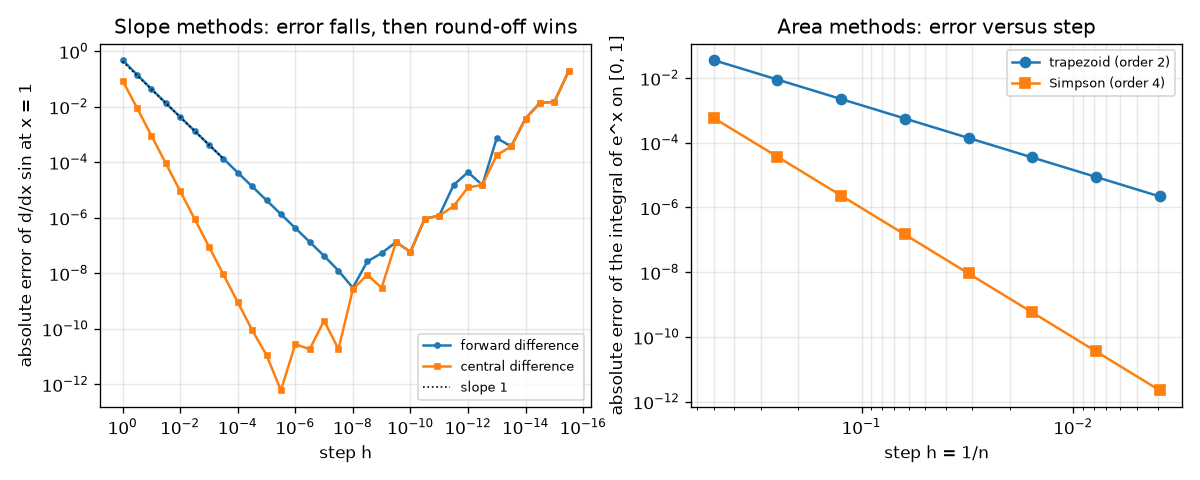
\includegraphics[width=0.85\linewidth]{figures/s03_error_vs_step.png}\\\small Left: slope errors fall with slopes 1 and 2 and then rise (round-off). Right: area errors fall with slopes 2 and 4.\end{center}

\subsection*{E. Worked example}
Find the forward and central difference of sin x at x = 1 with h = 0.1 and compare with the exact cos 1. Then find the trapezoid and Simpson areas of e\textasciicircum{}x on [0, 1] with n = 4 and compare with e - 1.
\begin{enumerate}[nosep]
\item Exact: cos 1 = 0.540302. Values: sin 1 = 0.841471, sin 1.1 = 0.891207, sin 0.9 = 0.783327.
\item Forward: (0.891207 - 0.841471) / 0.1 = 0.49736, error -0.0429. Central: (0.891207 - 0.783327) / 0.2 = 0.53940, error -0.0009. The central answer is about 48 times closer.
\item Areas: h = 0.25, values e\textasciicircum{}x = 1, 1.284025, 1.648721, 2.117000, 2.718282. Trapezoid: 0.25 * (0.5 + 1.284025 + 1.648721 + 2.117000 + 1.359141) = 1.727222, error +0.00894.
\item Simpson: (0.25 / 3) * (1 + 4 * 1.284025 + 2 * 1.648721 + 4 * 2.117000 + 2.718282) = 1.718319, error +0.000037. Exact e - 1 = 1.718282. Simpson is about 240 times closer with the same 5 points.
\item Pattern: with h = 0.01 the forward error is -0.0042 and the central error is -0.000009, in line with orders 1 and 2.
\end{enumerate}
\textbf{Answer.} Forward 0.49736 (error -0.0429) and central 0.53940 (error -0.0009); trapezoid 1.72722 (error 0.0089) and Simpson 1.71832 (error 0.000037).

\subsection*{F. Questions}
\begin{enumerate}[nosep]
\item \textbf{Conceptual.} Why can making the step h smaller make a numerical derivative worse?
\item \textbf{Numerical.} The trapezoid rule for e\textasciicircum{}x on [0, 1] with n = 16 has an error of 5.6e-4. Predict the error with n = 32, and for Simpson's rule if its error at n = 16 is 1.5e-7.
\item \textbf{Graph and simulation interpretation.} On a log-log plot of error against h, a method's points lie on a line which falls 4 decades while h falls 1 decade. What is its order? Which of our four methods is it?
\item \textbf{Design and optimisation challenge.} Design: you must integrate a function with one very narrow spike (width 0.005) on [0, 1] to 1e-8. Compare a uniform Simpson rule with an adaptive one, and say what could go wrong with the adaptive rule.
\end{enumerate}

\section{Session 4: Romberg integration: far more accuracy from the same function values}

\subsection*{A. Real-world problem}
Some numbers are expensive. If each function value is a one-minute simulation, or one reading from a slow instrument, you want the most accuracy from the fewest values. In Session 3, Simpson's rule with 17 values gave an error of about 1.5e-7 for the area under e\textasciicircum{}x on [0, 1]. Can the same 17 values give an error below 1e-12? And how much does that save when the function is a bell curve whose area needs to be known to ten digits? (Educational model with exact answers: not for design work.)

\subsection*{B. Concept and theory}
The trapezoid rule with 2\textasciicircum{}i slices is T\_i. Going from T\_(i-1) to T\_i needs only the new midpoints, so a table of \texttt{levels} rows costs 2\textasciicircum{}(levels-1) + 1 function values in total, the cost of one trapezoid rule on the finest grid.

For a smooth function the trapezoid error is a series in even powers of the step: T(h) = I + c1 h\textasciicircum{}2 + c2 h\textasciicircum{}4 + c3 h\textasciicircum{}6 + ..., where the constants c1, c2, ... do not depend on h. Halving h divides the h\textasciicircum{}2 term by 4, so the combination (4 T(h/2) - T(h)) / 3 cancels it and leaves an error of order h\textasciicircum{}4. This combination is exactly Simpson's rule. The same trick on two Simpson values (16 and 15 in place of 4 and 3) cancels the h\textasciicircum{}4 term, and so on. This is \textbf{Richardson extrapolation}; applying it to trapezoid sums is \textbf{Romberg integration}. Column j of the table has error about h\textasciicircum{}(2j+2) and is exact for polynomials up to degree 2j + 1.

The method depends on that series. If the function is not smooth (a square root at the end of the interval) the powers are not even integers and extrapolation gains little. If the function is smooth and periodic over the interval, the trapezoid rule is already extremely accurate, there is nothing left to cancel, and extrapolation only mixes in round-off. Finally, the usual stopping rule (stop when two successive corners agree) can be fooled when the first few values happen to agree by accident. Everything here has an exact answer to compare with; it is a teaching model, not a validated library.

\begin{itemize}[nosep]
\item h: step size, (b - a) / 2\textasciicircum{}i (same unit as x)
\item T\_i: trapezoid sum with 2\textasciicircum{}i slices (same unit as the integral)
\item R(i, j): Romberg table entry in row i and column j (R(i, 0) = T\_i) (same unit as the integral)
\item c1, c2, ...: error constants that do not depend on h (various)
\item levels: number of rows of the table (no unit)
\item values: number of function evaluations, 2\textasciicircum{}(levels-1) + 1 (no unit)
\end{itemize}

\begin{equation*}
T(h)=I+c_1h^2+c_2h^4+c_3h^6+\dots
\end{equation*}

\begin{equation*}
R(i,j)=\frac{4^{j}\,R(i,j-1)-R(i-1,j-1)}{4^{j}-1},\qquad R(i,0)=T_i
\end{equation*}

\begin{equation*}
R(i,1)=\frac{4\,T_i-T_{i-1}}{3}=\text{Simpson's rule with }2^i\text{ slices},\qquad \text{values}=2^{\,\mathrm{levels}-1}+1
\end{equation*}

\begin{center}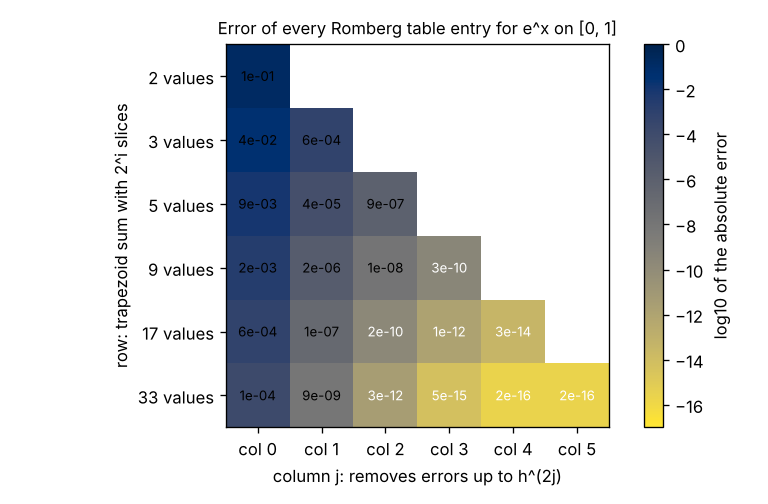
\includegraphics[width=0.7\linewidth]{figures/s04_romberg_table.png}\\\small The error of every entry of the Romberg table for e to the x on [0, 1] (darker is smaller).\end{center}

\begin{center}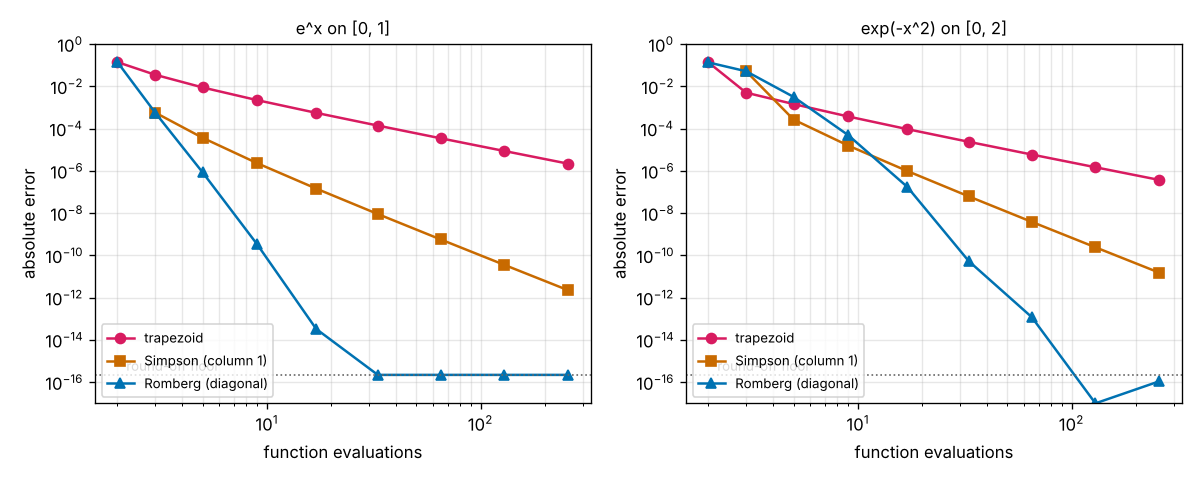
\includegraphics[width=0.95\linewidth]{figures/s04_error_vs_evaluations.png}\\\small Error against the number of function values: trapezoid, Simpson and Romberg, for e to the x and for the bell curve.\end{center}

\begin{center}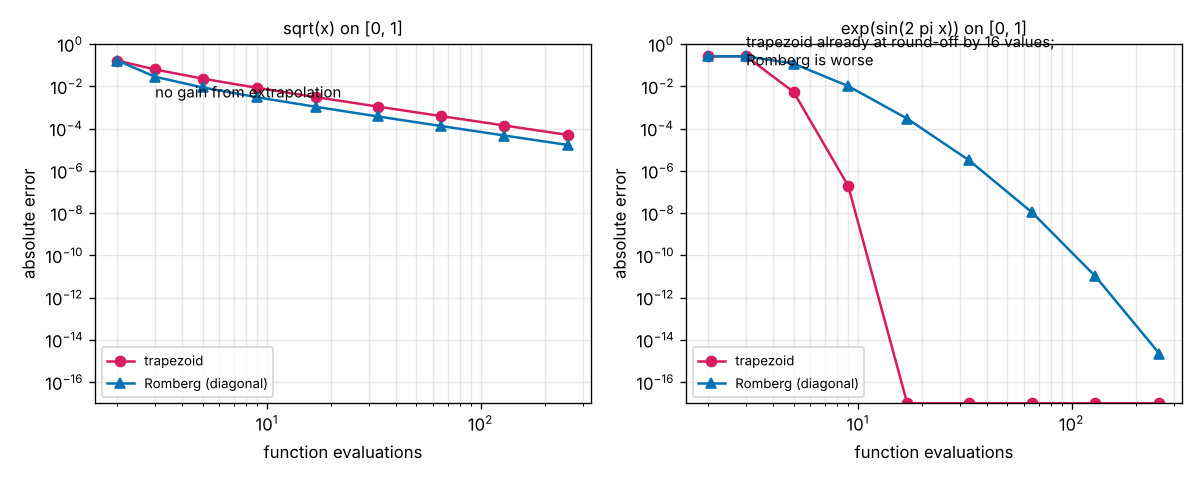
\includegraphics[width=0.95\linewidth]{figures/s04_failure_cases.png}\\\small Failure cases: the square root gains almost nothing, and for a periodic function Romberg is worse than the trapezoid rule.\end{center}

\subsection*{E. Worked example}
Build a three-row Romberg table for the area of e\textasciicircum{}x on [0, 1] and compare its corner with Simpson's rule for the same function values.
\begin{enumerate}[nosep]
\item Exact: e - 1 = 1.718282. The trapezoid rule with 1, 2 and 4 slices gives T0 = 0.5 (1 + 2.718282) = 1.859141, T1 = 1.753931 and T2 = 1.727222. The three sums use only 5 function values (2, then 1 new, then 2 new).
\item First column of corrections: R(1,1) = (4 x 1.753931 - 1.859141) / 3 = 1.718861 (error +5.8e-4) and R(2,1) = (4 x 1.727222 - 1.753931) / 3 = 1.718319 (error +3.7e-5).
\item R(2,1) is Simpson's rule with 4 slices: the same number you found in Session 3.
\item Second column: R(2,2) = (16 x 1.718319 - 1.718861) / 15 = 1.718283.
\item The error of R(2,2) is +8.6e-7. With the same 5 values the trapezoid rule has an error of 8.9e-3 (10 000 times larger) and Simpson 3.7e-5 (43 times larger).
\end{enumerate}
\textbf{Answer.} R(2,2) = 1.718283 with error 8.6e-7 from 5 function values, against Simpson's 1.718319 (error 3.7e-5) and the trapezoid rule's 1.727222 (error 8.9e-3).

\subsection*{F. Questions}
\begin{enumerate}[nosep]
\item \textbf{Conceptual.} Why does (4 T(h/2) - T(h)) / 3 remove the h\textasciicircum{}2 error of the trapezoid rule, and why do we divide by 3?
\item \textbf{Numerical.} The trapezoid rule for pi = the area of 4 / (1 + x\textasciicircum{}2) on [0, 1] gives T0 = 3.000000, T1 = 3.100000 and T2 = 3.131176. Complete the Romberg table (R(1,1), R(2,1), R(2,2)) and say which entry is closest to pi = 3.141593.
\item \textbf{Graph and simulation interpretation.} In the error-against-values figure for e\textasciicircum{}x, at 17 values the errors are 5.6e-4 (trapezoid), 1.5e-7 (Simpson) and 3.3e-14 (Romberg). By what factor is Romberg better than each, and what happens to its line beyond 33 values?
\item \textbf{Design and optimisation challenge.} Your budget is 40 function values (40 minutes) for the area of exp(-x\textasciicircum{}2) on [0, 2]. On the grids of 2\textasciicircum{}k + 1 values, which rule should you use and what error will it reach? What must you budget if you need 1e-12?
\end{enumerate}

\section{Session 5: Gaussian quadrature: choosing where to sample}

\subsection*{A. Real-world problem}
In Session 4 Romberg integration needed 65 function values to reach 1e-12 for a bell curve, and Simpson's rule needed 513. If every value is a one-minute simulation, that is a long wait. All those rules used equally spaced points and chose only the weights. What if we also choose where to sample? With 5 well-placed values the area of e\textasciicircum{}x on [0, 1] can be found with an error of 6.5e-13, while Simpson's rule with 5 values has an error of 3.7e-5. (Educational model with exact answers: not for design work.)

\subsection*{B. Concept and theory}
A quadrature rule approximates an integral by a weighted sum of function values: the area is about w\_1 f(x\_1) + ... + w\_n f(x\_n). With equally spaced points only the n weights are free, and the best you can do is be exact for polynomials of degree about n - 1. If the n points are free too there are 2n numbers to choose, and a polynomial of degree 2n - 1 has 2n coefficients. Gauss showed that the choice that makes the rule exact for all of them puts the points at the roots of the Legendre polynomial P\_n. These polynomials follow the recurrence (k + 1) P\_(k+1)(x) = (2k + 1) x P\_k(x) - k P\_(k-1)(x), starting from P\_0 = 1 and P\_1 = x. The roots lie inside the interval, crowd towards its ends and are symmetric; the weights are all positive and add up to the interval length (2 on [-1, 1]).

On [a, b] the points are mapped as x = m + r t, with the midpoint m = (a + b) / 2 and half-length r = (b - a) / 2, and the integral is r times the weighted sum. The 2-point rule has t = plus or minus 1/sqrt(3) with weights 1 and 1; the 3-point rule has t = 0 and plus or minus sqrt(3/5) with weights 8/9 and 5/9. For a function that is smooth enough (analytic) the error falls faster than any power of 1/n: every extra point adds several digits, which is why 5 points can beat 513.

There is a price. The rules are not nested: the (n + 1)-point rule shares almost no points with the n-point rule, so if you do not know in advance which n is enough and try n = 2, 3, 4, ... until two rules agree, every rule you try costs n new values. And, like all high-order rules, the method relies on smoothness: for sqrt(x) the error only falls like n\textasciicircum{}-3, for a periodic function the plain trapezoid rule is much better, and a narrow peak is simply missed. Everything here has an exact answer to compare with; it is a teaching model, not a validated library.

\begin{itemize}[nosep]
\item n: number of points (and function values) (no unit)
\item t\_i, w\_i: node and weight on [-1, 1] (roots of P\_n) (no unit)
\item m, r: midpoint and half-length of [a, b] (same unit as x)
\item P\_n: Legendre polynomial of degree n (no unit)
\item degree: highest power of x the rule integrates exactly, 2n - 1 (no unit)
\item values: number of function evaluations (no unit)
\end{itemize}

\begin{equation*}
\int_a^b f\,dx\approx r\sum_{i=1}^{n}w_i\,f(m+r\,t_i),\qquad m=\tfrac{a+b}2,\ r=\tfrac{b-a}2
\end{equation*}

\begin{equation*}
(k+1)P_{k+1}(x)=(2k+1)\,x\,P_k(x)-k\,P_{k-1}(x),\qquad P_n(t_i)=0,\qquad w_i=\frac{2}{(1-t_i^2)\,P_n'(t_i)^2}
\end{equation*}

\begin{equation*}
\int_{-1}^{1}x^k\,dx=\sum_i w_i t_i^k\ \ \text{for all }k\le 2n-1
\end{equation*}

\begin{center}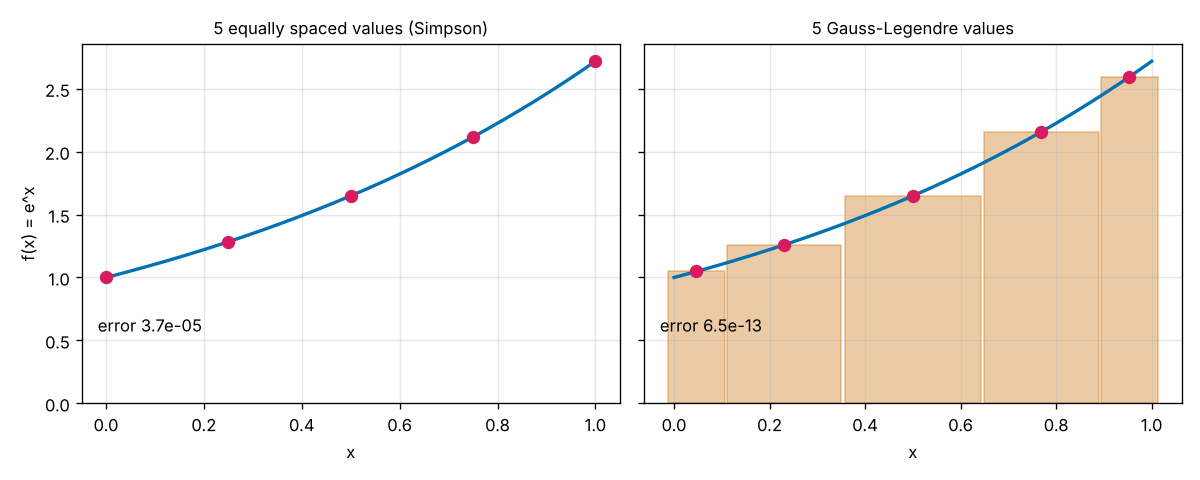
\includegraphics[width=0.95\linewidth]{figures/s05_nodes_weights.png}\\\small Five equally spaced values against the five Gauss-Legendre values for e to the x on [0, 1]; the rectangles show the weights.\end{center}

\begin{center}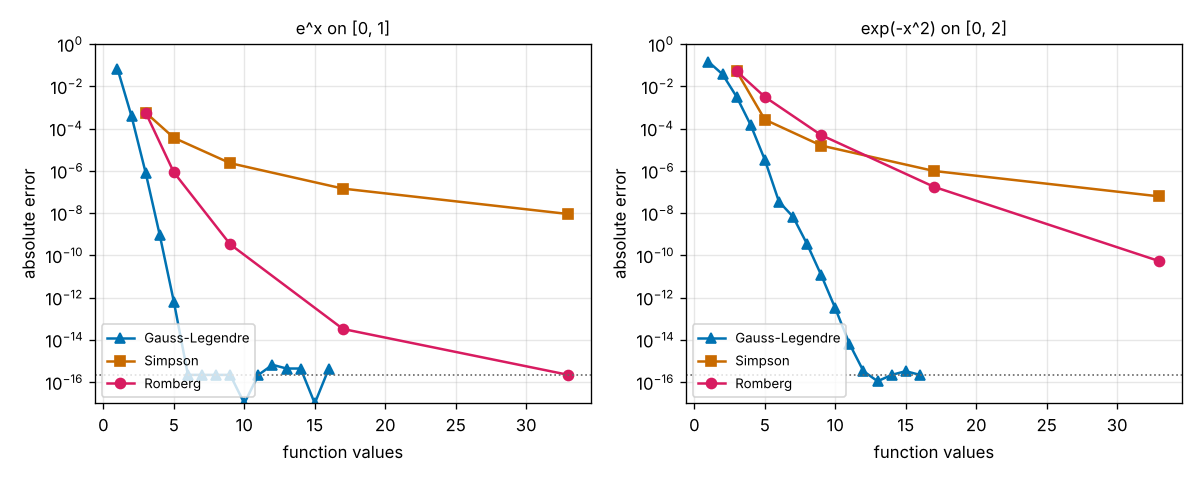
\includegraphics[width=0.95\linewidth]{figures/s05_error_vs_values.png}\\\small Error against the number of function values for Simpson, Romberg and Gauss, on e to the x and on the bell curve.\end{center}

\begin{center}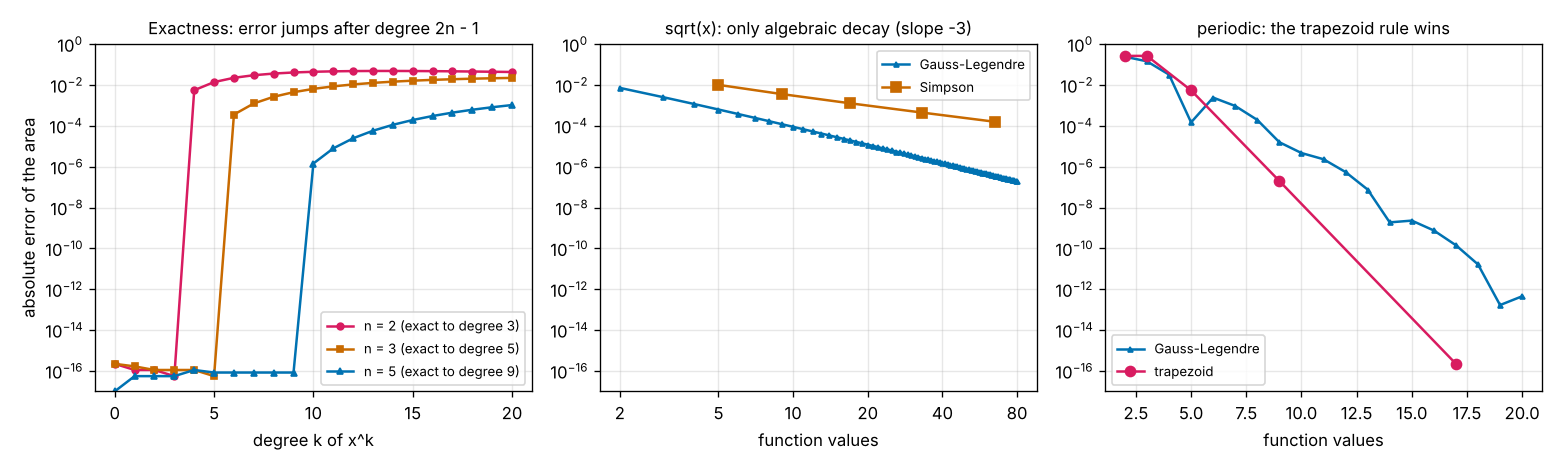
\includegraphics[width=1.0\linewidth]{figures/s05_exactness_and_failures.png}\\\small Left: the error jumps after degree 2n minus 1. Middle: the square root converges slowly. Right: for a periodic function the trapezoid rule wins.\end{center}

\subsection*{E. Worked example}
Find the area of e\textasciicircum{}x on [0, 1] with the 2-point and the 3-point Gauss-Legendre rules and compare with Simpson's rule for the same number of function values.
\begin{enumerate}[nosep]
\item Exact: e - 1 = 1.718282. On [0, 1] the midpoint is m = 0.5 and the half-length r = 0.5.
\item Two points: t = plus or minus 0.577350, so x = 0.5 plus or minus 0.288675 = 0.211325 and 0.788675, with weights 1 and 1. The values are e\textasciicircum{}0.211325 = 1.235314 and e\textasciicircum{}0.788675 = 2.200479.
\item Two-point area: 0.5 x (1 x 1.235314 + 1 x 2.200479) = 1.717896, error -3.9e-4.
\item Three points: t = -0.774597, 0 and 0.774597, so x = 0.112702, 0.5 and 0.887298, with weights 5/9, 8/9 and 5/9. The values are 1.119298, 1.648721 and 2.428560.
\item Three-point area: 0.5 x (5/9 x 1.119298 + 8/9 x 1.648721 + 5/9 x 2.428560) = 1.718281, error -8.2e-7.
\item Simpson's rule with the same 3 values (x = 0, 0.5, 1) gives 1.718861 with error +5.8e-4, so the 3-point Gauss rule is about 700 times closer.
\end{enumerate}
\textbf{Answer.} 2 points: 1.717896 (error -3.9e-4); 3 points: 1.718281 (error -8.2e-7), against Simpson's 1.718861 (error 5.8e-4) for the same 3 values.

\subsection*{F. Questions}
\begin{enumerate}[nosep]
\item \textbf{Conceptual.} Why is the n-point Gauss-Legendre rule exact up to degree 2n - 1, when the n-point rule with equally spaced points is exact only up to about degree n - 1?
\item \textbf{Numerical.} Use the 2-point Gauss-Legendre rule to find the area of x\textasciicircum{}3 + 1 on [1, 3], and then the area of x\textasciicircum{}4 on [1, 3]. The exact answers are 22 and 48.4.
\item \textbf{Graph and simulation interpretation.} In the error-against-values figure for the bell curve, at 9 values the errors are 1.6e-5 (Simpson), 5.0e-5 (Romberg) and 1.2e-11 (Gauss). What do you conclude about Gauss, and about the claim that Romberg is always better than Simpson?
\item \textbf{Design and optimisation challenge.} You can afford 10 function values (10 minutes) for the area of exp(-x\textasciicircum{}2) on [0, 2]. Which rule do you choose and what error do you expect? Then suppose you needed 1e-12 and did not know how many points to use: what would the Gauss approach cost, and how does it compare with Romberg?
\end{enumerate}

\section{Real-world mini-project}
\textbf{Reconstruct the distance travelled from a noisy speedometer log.} A car's speedometer was logged 10 times per second for 60 s with \texttt{t, v = speedometer\_log()} from Session 3 (fixed seed 4, the default; the figures below are for that seed and are asserted by the Session 3 checkpoint). The log has random noise of 0.8 m/s and the speedometer reads 2 percent too high. The only outside fact is that a pair of roadside markers shows the car covered 822 m in the 60 s. Use \texttt{integrate\_log} to reconstruct the distance, remove the calibration error with the marker fact, and then estimate the car's acceleration by smoothing the speed before differentiating (a moving average of 21 samples is a good start).

\textbf{How many function values does each rule need?} A heat-flow simulation returns the flux q(x) = exp(-x\textasciicircum{}2) (made-up units) at a point x on a plate 2 units wide, and every call costs one minute. The total heat is the integral of q from 0 to 2, whose exact value sqrt(pi)/2 erf(2) = 0.882081 is known here so that you can check. Use \texttt{evaluations\_needed} and \texttt{romberg\_table} from Session 4 to find, for the targets 1e-6, 1e-8, 1e-10 and 1e-12, how many function values (minutes) the trapezoid rule, Simpson's rule and Romberg integration need on the grids with 2\textasciicircum{}k + 1 values. \textbf{Deliverable:} A script that prints a table of values needed for each rule and target, the number of minutes saved by Romberg against Simpson at 1e-10, and a log-log plot of error against the number of values for the three rules; then two sentences on what happens to Romberg for sqrt(x) on [0, 1] with 129 values (use \texttt{FUNCTIONS[3]}) and why. \textbf{Success looks like:} For 1e-6, 1e-8, 1e-10 and 1e-12 Simpson needs 17, 65, 257 and 513 values and Romberg 17, 33, 33 and 65; the trapezoid rule needs 257, 2049 and 16385 and more than 131 073 for the last. At 1e-10 Romberg saves 224 minutes against Simpson. For sqrt(x) with 129 values the Romberg error is 4.7e-5, only 3 times better than the trapezoid rule's 1.4e-4, because the error series has no even powers of h to cancel.

\textbf{Which rule for an expensive simulation?} The plate of Session 4 again: a simulation returns the flux q(x) = exp(-x\textasciicircum{}2) (made-up units) at a point on a plate 2 units wide, one minute per call, and the total is the integral from 0 to 2 (exact 0.882081). Use \texttt{gauss\_values\_needed}, \texttt{gauss\_tol} and \texttt{gauss\_legendre} from Session 5 and the Session 4 counts of Simpson and Romberg (17, 65, 257, 513 and 17, 33, 33, 65 values for 1e-6, 1e-8, 1e-10 and 1e-12). Find, for those targets, the number of values Gauss needs when n is known and the total number it spends when n must be found by trying, then check what happens for the two functions that Gauss does not like. \textbf{Deliverable:} A script that prints the table of values for the three rules at the four targets (and the total spent by the stopping rule), a log-scale plot of error against values, and a recommendation in three sentences: which rule you would use for this plate, and for a square root \texttt{FUNCTIONS[3]} and for a periodic function \texttt{FUNCTIONS[4]} over one period. \textbf{Success looks like:} Gauss needs 6, 7, 9 and 10 values when n is known, but the stopping rule spends 27, 35, 54 and 65 (for 1e-12 the same 65 as Romberg, because the rules are not nested). For sqrt(x) 80 Gauss values give an error of 2.0e-7 (Romberg with 129 values: 4.7e-5), but 160 values still give only 2.5e-8, an order of 3 on a log-log plot. For the periodic function the plain trapezoid rule with 17 values is at round-off (2e-16) while Gauss with 17 values has an error of 1.4e-10.

\section{The path ahead}
\begin{enumerate}[nosep]
\item \textbf{Session 6: Derivatives without subtraction.} A derivative routine that avoids the round-off limit of Session 3.
\item \textbf{Session 7: Derivatives of noisy data.} A smoothing differentiator for the speedometer log of the mini-project.
\item \textbf{Session 8: Solve the braking ODE.} A solver for a braking car with drag, v' = -c v\textasciicircum{}2, and the distance it travels.
\end{enumerate}

\section{Answers and hints}

\subsection*{Session 1}
\begin{enumerate}[nosep]
\item \textbf{Conceptual.} Hint: Read the height of the speed graph, not its steepness, and remember slope = speed. Solution: No. A flat speed graph at 10 m/s means a constant speed of 10 m/s: the car is moving steadily, its distance graph is a straight sloped line (slope 10 m/s). A flat distance graph means the distance is not changing, so the speed is zero and the car is stopped. 'Flat' means different things on the two graphs: the speed graph shows the speed itself, the distance graph shows it only through its slope.
\item \textbf{Numerical.} Hint: Add three trapezoids; average speed is total distance divided by total time. Solution: Slice 1: (0 + 12)/2 * 2 = 12 m. Slice 2: (12 + 12)/2 * 2 = 24 m. Slice 3: (12 + 6)/2 * 2 = 18 m. Total = 54 m. Average speed = 54 m / 6 s = 9 m/s. Sanity check: the speed is always between 0 and 12 m/s, so 9 m/s is a believable average. Units: m/s * s = m.
\item \textbf{Graph and simulation interpretation.} Hint: The slope of the distance graph at a time equals the speed at that time. Solution: The curve is steepest at t = 4 s where the speed peaks at 14 m/s, so the slope is 14 m/s. At t = 6 s the speed is 6 m/s, so the slope has dropped to 6 m/s: the curve is still rising but much more gently. The distance never goes down because the speed is never negative.
\item \textbf{Design and optimisation challenge.} Hint: The total distance is 2 v1 + 2 v2 + v3 (three trapezoids). Try the largest speeds first. Solution: Total = 2 v1 + 2 v2 + v3. With 20, 20, 20: 40 + 40 + 20 = 100 m, which works. With 20, 20, 10: 90 m, just enough. With 15, 15, 15: 30 + 30 + 15 = 75 m, which fails. The first two speeds count double because they belong to two slices each, so being fast early matters most; the trade-off is that finishing at 20 m/s leaves less margin for stopping. Assumption: straight-line speed changes, no reversing.
\end{enumerate}

\subsection*{Session 2}
\begin{enumerate}[nosep]
\item \textbf{Conceptual.} Hint: Where does the secant line touch the curve, and what does a limit do? Solution: The secant line touches the curve at two points, so it measures the average slope over the gap h; the tangent line touches at one point. For x = 3 t\textasciicircum{}2 + 2 t at t = 2 the secant slope is 14 + 3 h, which is never 14 for h \textgreater{} 0. But it gets as close as we like by making h small, and that limit is the derivative. Computing secants is how computers estimate derivatives when no formula is known (Session 3).
\item \textbf{Numerical.} Hint: Use d/dt of c t\textasciicircum{}n = c n t\textasciicircum{}(n-1) twice. Solution: x(3) = 5 * 9 + 4 * 3 = 45 + 12 = 57 m. v(t) = 10 t + 4, so v(3) = 34 m/s. a = 10 m/s\textasciicircum{}2. Units: x is in m, so 5 is m/s\textasciicircum{}2 (m/s\textasciicircum{}2 * s\textasciicircum{}2 = m) and 4 is m/s (m/s * s = m). v = 10 t + 4 then has 10 in m/s\textasciicircum{}2 and 4 in m/s: m/s\textasciicircum{}2 * s = m/s. All terms are consistent.
\item \textbf{Graph and simulation interpretation.} Hint: The secant slope equals v + A h. Solution: With v = 14 m/s and A = 3 m/s\textasciicircum{}2 the secant slope is 14 + 3 * 2 = 20 m/s; with h = 0.1 it is 14.3 m/s. The secant line rotates towards the red tangent line as h shrinks. The secant is steeper than the tangent because the curve bends upwards (positive acceleration).
\item \textbf{Design and optimisation challenge.} Hint: Use d = v0 t\_r + v0\textasciicircum{}2 / (2 a). For the second part solve v t\_r + v\textasciicircum{}2 / (2 a) = 40 for v. Solution: From 25 m/s: reaction distance 25 * 0.75 = 18.75 m and braking distance 625 / 12 = 52.08 m, total about 70.8 m, far more than 40 m. For 40 m: v\textasciicircum{}2 / 12 + 0.75 v - 40 = 0, i.e. v\textasciicircum{}2 + 9 v - 480 = 0, so v = (-9 + sqrt(81 + 1920)) / 2 = 17.87 m/s, about 64 km/h. Check: 17.87 * 0.75 + 17.87\textasciicircum{}2 / 12 = 13.4 + 26.6 = 40 m. The model leaves out that real deceleration depends on tyres, road surface, slope and load, and that reaction times vary; it is a classroom model, not driving advice. The braking part grows as v\textasciicircum{}2, so doubling the speed quadruples it.
\end{enumerate}

\subsection*{Session 3}
\begin{enumerate}[nosep]
\item \textbf{Conceptual.} Hint: Think about f(x + h) - f(x) when the two numbers agree in their first 12 digits. Solution: When h is tiny, f(x + h) and f(x) are almost equal, and subtracting them cancels the leading digits, leaving only the few digits that are uncertain because the computer keeps about 16. Dividing by the tiny h then magnifies that round-off error by 1 / h. The method (truncation) error falls with h but the round-off error rises, so the total error has a minimum. In our test the forward difference is best near h = 1e-8 (error 3e-9) and the central near h = 3e-6 (error 6e-13); at h = 1e-15 both give an error of about 0.19.
\item \textbf{Numerical.} Hint: Doubling n halves h; error scales as h\textasciicircum{}p, so it is divided by 2\textasciicircum{}p. Solution: Trapezoid is order 2, so the error falls by a factor 2\textasciicircum{}2 = 4: about 1.4e-4. Simpson is order 4, so the error falls by 2\textasciicircum{}4 = 16: about 9e-9. Sanity check: Simpson at n = 16 is already about 4000 times more accurate than the trapezoid at the same n (5.6e-4 against 1.5e-7).
\item \textbf{Graph and simulation interpretation.} Hint: Slope = change in log error / change in log h. Solution: The slope is 4 (error falls by a factor 10\textasciicircum{}4 when h falls by 10), so the order is 4: Simpson's rule. Forward difference has slope 1, central difference and the trapezoid rule have slope 2.
\item \textbf{Design and optimisation challenge.} Hint: The adaptive rule splits slices only where its two estimates disagree. What if the first few samples all miss the spike? Solution: For the peak at 0.35 with width 0.005 the exact area is 0.0088623. Uniform Simpson reaches 1e-8 only with n = 512 slices (513 evaluations). Adaptive Simpson starting from 16 panels reaches the same accuracy with 424 evaluations, putting small slices at the spike. The risk: if the starting samples all miss the spike, the two estimates agree (both near 0) and the rule stops early with the wrong answer; that is why we start from 16 panels. The saving is moderate here and larger for narrower features. A 10-slice trapezoid reports 0.000000, wrong by 100 percent.
\end{enumerate}

\subsection*{Session 4}
\begin{enumerate}[nosep]
\item \textbf{Conceptual.} Hint: Write T(h) = I + c1 h\textasciicircum{}2 + ... and T(h/2) = I + c1 h\textasciicircum{}2 / 4 + ... and look at the c1 terms. Solution: T(h) = I + c1 h\textasciicircum{}2 + c2 h\textasciicircum{}4 + ... and, with half the step, T(h/2) = I + c1 h\textasciicircum{}2 / 4 + c2 h\textasciicircum{}4 / 16 + .... The h\textasciicircum{}2 term of 4 T(h/2) is c1 h\textasciicircum{}2, the same as in T(h), so it cancels in 4 T(h/2) - T(h). What remains is 3 I plus terms in h\textasciicircum{}4, so we divide by 3 to get I back. The leftover error is order h\textasciicircum{}4: this is Simpson's rule. For the next column the h\textasciicircum{}4 terms are c2 h\textasciicircum{}4 and c2 h\textasciicircum{}4 / 16, so the factor is 16 and the divisor 15.
\item \textbf{Numerical.} Hint: R(i,1) = (4 T\_i - T\_(i-1)) / 3 and R(2,2) = (16 R(2,1) - R(1,1)) / 15. Solution: R(1,1) = (4 x 3.1 - 3.0) / 3 = 3.133333. R(2,1) = (4 x 3.131176 - 3.1) / 3 = 3.141569. R(2,2) = (16 x 3.141569 - 3.133333) / 15 = 3.142118. The errors are -8.3e-3, -2.4e-5 and +5.3e-4: the closest entry is R(2,1), not the corner. With only 5 values the h\textasciicircum{}6 term is not yet small compared with the h\textasciicircum{}4 term, so the last extrapolation overshoots. With 6 rows (33 values) the corner has caught up and is at 4.8e-11, but it is no better than the best entry of its row (3.7e-11).
\item \textbf{Graph and simulation interpretation.} Hint: Divide the errors. Look for the floor in the figure near 1e-16. Solution: Romberg is 5.6e-4 / 3.3e-14 = 1.7e10 times better than the trapezoid rule and 1.5e-7 / 3.3e-14 = 4.4e6 times better than Simpson. Beyond 33 values (error about 2e-16 in the lesson) the line stops falling and wobbles around 1e-16: the answer is at the round-off limit of double precision, so more values cannot help and cost more.
\item \textbf{Design and optimisation challenge.} Hint: The grids have 3, 5, 9, 17, 33, 65 values. Use the largest that fits, and the table in section C. Solution: The largest grid within 40 values has 33 values. There the errors are 2.4e-5 for the trapezoid rule, 6.2e-8 for Simpson and 5.3e-11 for Romberg (corner), so Romberg is the best choice, over 1000 times better than Simpson. For 1e-12 Romberg needs 65 values (error 1.2e-13) against 513 for Simpson, so budget 65 minutes. Note that for this function the corner is not always the best entry of its row: at 33 values the entry in column 2 has error 2.2e-11, slightly better than the corner, but you cannot know which entry is best without the exact answer, so the corner is the usual choice.
\end{enumerate}

\subsection*{Session 5}
\begin{enumerate}[nosep]
\item \textbf{Conceptual.} Hint: Count the free numbers in a rule (points and weights) and the coefficients of a polynomial. Solution: A rule with n fixed equally spaced points can only choose its n weights, so it can be made exact for the n monomials 1, x, ..., x\textasciicircum{}(n-1): degree n - 1 (one more for symmetric rules such as Simpson's). If the n points are free as well there are 2n numbers to choose, and a polynomial of degree 2n - 1 has exactly 2n coefficients, so all of them can be integrated exactly. The Legendre roots are the choice that achieves this. Check: the 3-point rule is exact for x\textasciicircum{}5 but not for x\textasciicircum{}6, where its error on [0, 1] is 3.6e-4.
\item \textbf{Numerical.} Hint: The midpoint is m = 2 and the half-length r = 1, so x = 2 plus or minus 0.57735 and the weights are 1 and 1. Solution: The points are x = 2 - 0.577350 = 1.422650 and 2 + 0.577350 = 2.577350. For x\textasciicircum{}3 + 1 the values are 3.879348 and 18.120648; the area is 1 x (3.879348 + 18.120648) = 22.000 (exact: a cubic is within degree 2n - 1 = 3). For x\textasciicircum{}4 the values are 4.0963 and 44.1259, the area is 48.2222, an error of -0.178: degree 4 is beyond 2n - 1, so the rule is no longer exact.
\item \textbf{Graph and simulation interpretation.} Hint: Divide the errors, and compare Romberg with Simpson at the same number of values. Solution: Gauss is 1.6e-5 / 1.2e-11 = 1.4e6 times better than Simpson with the same 9 values. At 9 values Romberg (corner) is about 3 times worse than Simpson: the bell curve bends so much that the higher columns of the table, which assume the h\textasciicircum{}2, h\textasciicircum{}4, h\textasciicircum{}6 error series has already settled, make things worse until the grid is fine enough. At 17 values Romberg wins (1.8e-7 against 9.9e-7). So Romberg is not always better than Simpson, and the corner of a table is a good choice only once the grid is fine.
\item \textbf{Design and optimisation challenge.} Hint: Use the table in section C: for the second part count all the values spent by trying n = 2, 3, 4, ... Solution: With 10 values: Gauss with n = 10 has an error of 3.1e-13, Simpson with 9 values has 1.6e-5 and Romberg with 9 values 5.0e-5: choose Gauss. If you do not know n in advance you raise n until two rules agree to within 1e-12; that happens at n = 11 after 2 + 3 + ... + 11 = 65 values in total, exactly what Romberg needs (65), because the Gauss rules are not nested and nothing is reused. Gauss wins clearly when you can fix n in advance (for example from a trial run on a similar problem), and its advantage largely disappears when you must discover n during the run.
\end{enumerate}

\section{How to join}
Read \texttt{CONTRIBUTING.md} in the repository, then pick an issue labelled \texttt{good first issue}. Repository: \url{https://github.com/KrunalPanchal1995/pan-iit-oss/tree/main/opencalculus}

\end{document}
